\documentclass[10pt,aspectratio=169]{beamer}
\usetheme[progressbar=frametitle,numbering=fraction,block=fill]{metropolis}
\usepackage[T1]{fontenc}
\usepackage{amsmath,amssymb,bm,booktabs,tabularx,array,colortbl}
\usepackage{tikz}
\usetikzlibrary{arrows.meta,positioning,shapes.geometric,fit,backgrounds,calc,shadows}
\usepackage{xcolor}
\usepackage{listings}

% ------------------------------------------------------------------ palette
\definecolor{navy}{HTML}{23373B}
\definecolor{tealx}{HTML}{14857A}
\definecolor{orangex}{HTML}{EB811B}
\definecolor{softbg}{HTML}{F4F6F6}
% colour code for physical quantities (used consistently in all equations)
\definecolor{cSpin}{HTML}{1F5FAD}    % spins S, sigma
\definecolor{cMaj}{HTML}{C0392B}     % matter Majoranas c
\definecolor{cGauge}{HTML}{E67E22}   % gauge Majoranas b, gauge field u
\definecolor{cCoup}{HTML}{2E8B57}    % couplings J, K, Gamma, kappa, h
\definecolor{cFlux}{HTML}{7D3C98}    % fluxes W_p, Wilson loops, Phi
\definecolor{cEn}{HTML}{14857A}      % energies E, epsilon, omega
\definecolor{cMom}{HTML}{8B5A2B}     % momenta k, q
\definecolor{cEnt}{HTML}{C2185B}     % entropies S_A, gamma
\definecolor{cWf}{HTML}{23373B}      % wave functions, projectors

\newcommand{\Sp}[1]{{\color{cSpin}#1}}
\newcommand{\Mj}[1]{{\color{cMaj}#1}}
\newcommand{\Ga}[1]{{\color{cGauge}#1}}
\newcommand{\Cp}[1]{{\color{cCoup}#1}}
\newcommand{\Fx}[1]{{\color{cFlux}#1}}
\newcommand{\En}[1]{{\color{cEn}#1}}
\newcommand{\Mo}[1]{{\color{cMom}#1}}
\newcommand{\Et}[1]{{\color{cEnt}#1}}
\newcommand{\Wf}[1]{{\color{cWf}#1}}
\newcommand{\vk}{\Mo{\mathbf k}}
\newcommand{\vq}{\Mo{\mathbf q}}

\setbeamercolor{frametitle}{bg=navy}
\setbeamercolor{progress bar}{fg=orangex,bg=orangex!20}
\setbeamercolor{block title}{bg=navy!12,fg=navy}
\setbeamercolor{block body}{bg=softbg}
\setbeamercolor{block title alerted}{bg=orangex!25,fg=navy}
\setbeamercolor{block body alerted}{bg=orangex!6}
\setbeamercolor{block title example}{bg=tealx!20,fg=navy}
\setbeamercolor{block body example}{bg=tealx!5}
\metroset{titleformat=smallcaps,sectionpage=none}

\lstset{basicstyle=\ttfamily\scriptsize,keywordstyle=\color{tealx}\bfseries,commentstyle=\color{gray},
  stringstyle=\color{orangex},backgroundcolor=\color{softbg},frame=none,columns=fullflexible,
  keepspaces=true,showstringspaces=false,language=Python,morekeywords={import,from,as},xleftmargin=4pt,
  aboveskip=2pt,belowskip=2pt}

\tikzset{
  box/.style={rounded corners=4pt,draw=#1!70,fill=#1!10,minimum height=0.8cm,text width=2.35cm,align=center,font=\scriptsize},
  big/.style={rounded corners=5pt,draw=navy,fill=navy,text=white,minimum height=0.95cm,text width=3.3cm,align=center,font=\small\bfseries},
  arr/.style={-{Stealth[length=2.3mm]},line width=0.9pt,color=navy!70}}
\newcommand{\pill}[2][tealx]{\tikz[baseline=(t.base)]\node[rounded corners=3pt,fill=#1!15,draw=#1!60,inner sep=2pt,font=\scriptsize\bfseries,text=navy](t){#2};}
\newcommand{\ok}{{\color{tealx}\checkmark}}

\title{qslab}
\subtitle{A laboratory for quantum spin liquids\\[2pt]\small exact diagonalisation $\cdot$ Majorana $\cdot$ stabilizers $\cdot$ partons/VMC $\cdot$ DMRG $\cdot$ neural quantum states}
\author{Gokaran Shukla}
\institute{King Abdullah University of Science and Technology (KAUST)\\[2pt]\href{https://github.com/Gokaran-Shukla/qslab}{\texttt{github.com/Gokaran-Shukla/qslab}}}
\date{November 2026}

\begin{document}

% =================================================================== title
{
\setbeamertemplate{background}{%
\begin{tikzpicture}[remember picture,overlay]
  \begin{scope}[shift={($(current page.south east)+(-4.6,0.55)$)},scale=0.42]
    \foreach \cx/\cy in {0/0,1.732/0,3.464/0,5.196/0,0.866/1.5,2.598/1.5,4.330/1.5,6.062/1.5,1.732/3,3.464/3,5.196/3}{
      \begin{scope}[shift={(\cx,\cy)}]
        \draw[line width=1.5pt,cSpin!85] (0,1) -- (0.866,0.5);   \draw[line width=1.5pt,cCoup!85] (0.866,0.5) -- (0.866,-0.5);
        \draw[line width=1.5pt,cMaj!85] (0.866,-0.5) -- (0,-1);  \draw[line width=1.5pt,cSpin!85] (0,-1) -- (-0.866,-0.5);
        \draw[line width=1.5pt,cCoup!85] (-0.866,-0.5) -- (-0.866,0.5); \draw[line width=1.5pt,cMaj!85] (-0.866,0.5) -- (0,1);
        \foreach \a in {90,210,330}{\fill[navy] (\a:1) circle (3.2pt);}
        \foreach \a in {30,150,270}{\fill[orangex] (\a:1) circle (3.2pt);}
        \node[cFlux!70,font=\tiny] at (0,0) {$W_p$};
      \end{scope}}
  \end{scope}
\end{tikzpicture}}
\maketitle
}

% =================================================================== outline
\begin{frame}{Outline}
\begin{columns}[T]
\column{0.48\textwidth}
\begin{enumerate}
\item Why simulate spin liquids?
\item Architecture: one operator algebra, many solvers
\item Exact diagonalisation and Hilbert-space engineering
\item Kitaev honeycomb: exact Majorana solution
\item Kitaev materials: J--K--$\Gamma$--$\Gamma'$
\item Toric code and topological entanglement
\end{enumerate}
\column{0.48\textwidth}
\begin{enumerate}\setcounter{enumi}{6}
\item Kagome and triangular antiferromagnets
\item Partons, Gutzwiller projection, VMC
\item DMRG and neural quantum states
\item Dynamics and thermodynamics
\item Parallel computing: node, MPI, GPU
\item Validation, tutorials and quizzes
\end{enumerate}
\end{columns}
\vfill
\begin{block}{Colour code used in every equation}
\small
\Sp{spins $S,\sigma$}\quad \Mj{Majoranas $c$}\quad \Ga{gauge $b,u$}\quad \Cp{couplings $J,K,\Gamma,\kappa,h$}\quad
\Fx{fluxes $W_p$}\quad \En{energies $E,\varepsilon,\omega$}\quad \Mo{momenta $\mathbf k,\mathbf q$}\quad \Et{entropies $S_A,\gamma$}
\end{block}
\end{frame}

% =================================================================== motivation
\section{Why simulate spin liquids?}
\begin{frame}{A quantum spin liquid is defined by what it is \emph{not}, so we need many probes}
\begin{columns}[T]
\column{0.5\textwidth}
\begin{block}{Signatures}
\begin{itemize}\small
\item no magnetic order: $\langle\Sp{\mathbf S_i}\rangle=0$, no Bragg peak in $S(\vq)$ as $N\to\infty$
\item fractionalised excitations (spinons, visons, Majoranas), seen as continua in $S(\vq,\En{\omega})$
\item topological order: torus degeneracy, $\Et{S_A}=\alpha|\partial A|-\Et{\gamma}$
\item emergent gauge field: conserved fluxes $\Fx{W_p}$
\item thermodynamic fingerprints: entropy plateaus, multiple peaks in $C(T)$
\end{itemize}
\end{block}
\column{0.47\textwidth}
\begin{alertblock}{No single method suffices}
\small
\begin{tabular}{@{}ll@{}}
ED & exact, but small $N$\\
QMC & sign problem when frustrated\\
DMRG & 1D or narrow cylinders\\
VMC/partons & biased by the ansatz\\
NQS & sign structure is hard\\
\end{tabular}
\end{alertblock}
\begin{exampleblock}{qslab's approach}
\small One Hamiltonian object, six solvers, and cross-checks between them.
Every number is benchmarked against an exact or published result.
\end{exampleblock}
\end{columns}
\end{frame}

% =================================================================== architecture
\section{Architecture}
\begin{frame}{One operator algebra, many solvers}
\centering
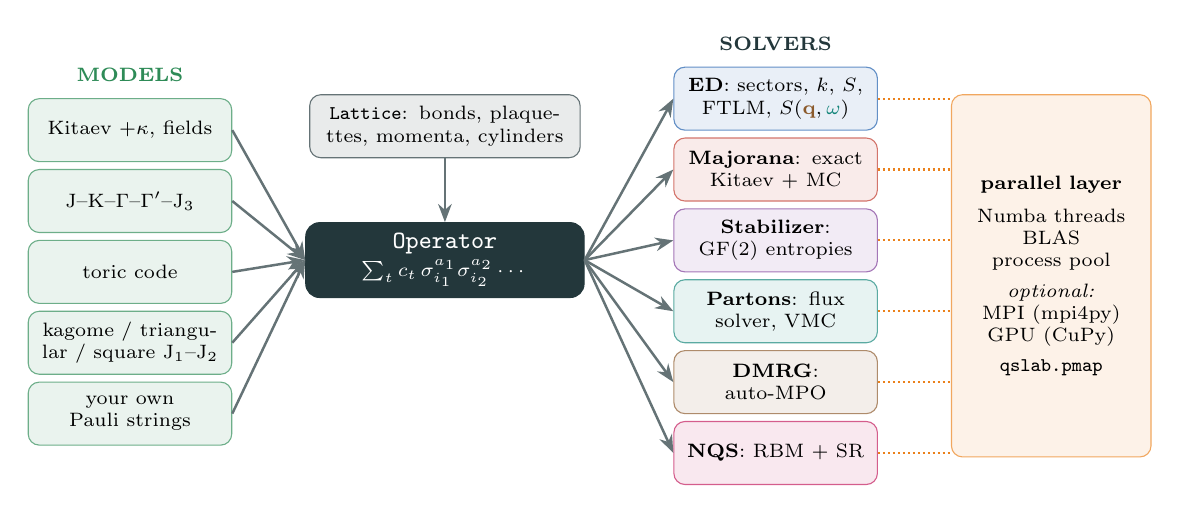
\begin{tikzpicture}
\node[box=cCoup] (m1) at (-5.6,1.65) {Kitaev $+\kappa$, fields};
\node[box=cCoup] (m2) at (-5.6,0.75) {J--K--$\Gamma$--$\Gamma'$--J$_3$};
\node[box=cCoup] (m3) at (-5.6,-0.15) {toric code};
\node[box=cCoup] (m4) at (-5.6,-1.05) {kagome / triangular / square J$_1$--J$_2$};
\node[box=cCoup] (m5) at (-5.6,-1.95) {your own Pauli strings};
\node[font=\scriptsize\bfseries,text=cCoup] at (-5.6,2.35) {MODELS};
\node[big] (op) at (-1.6,0) {\texttt{Operator}\\[-1pt]{\scriptsize\mdseries $\sum_t c_t\,{\color{white}\sigma^{a_1}_{i_1}\sigma^{a_2}_{i_2}}\cdots$}};
\node[box=navy,text width=3.2cm] (lat) at (-1.6,1.7) {\texttt{Lattice}: bonds, plaquettes, momenta, cylinders};
\foreach \i in {1,...,5}{\draw[arr] (m\i.east) -- (op.west);}
\draw[arr] (lat) -- (op);
\node[box=cSpin] (s1) at (2.6,2.05) {\textbf{ED}: sectors, $k$, $S$, FTLM, $S(\vq,\En\omega)$};
\node[box=cMaj] (s2) at (2.6,1.15) {\textbf{Majorana}: exact Kitaev + MC};
\node[box=cFlux] (s3) at (2.6,0.25) {\textbf{Stabilizer}: GF(2) entropies};
\node[box=cEn] (s4) at (2.6,-0.65) {\textbf{Partons}: flux solver, VMC};
\node[box=cMom] (s5) at (2.6,-1.55) {\textbf{DMRG}: auto-MPO};
\node[box=cEnt] (s6) at (2.6,-2.45) {\textbf{NQS}: RBM + SR};
\node[font=\scriptsize\bfseries,text=navy] at (2.6,2.75) {SOLVERS};
\foreach \i in {1,...,6}{\draw[arr] (op.east) -- (s\i.west);}
\node[box=orangex,text width=2.3cm,minimum height=4.6cm] (par) at (6.1,-0.2) {\textbf{parallel layer}\\[4pt]Numba threads\\BLAS\\process pool\\[3pt]\emph{optional:}\\MPI (mpi4py)\\GPU (CuPy)\\[3pt]\texttt{qslab.pmap}};
\foreach \i in {1,...,6}{\draw[densely dotted,color=orangex,line width=0.8pt] (s\i.east) -- (par.west|-s\i.east);}
\end{tikzpicture}
\end{frame}

\begin{frame}[fragile]{Every Hamiltonian is a sum of Pauli strings}
\begin{columns}[T]
\column{0.52\textwidth}
\footnotesize
Basis state $=$ integer $n$; bit $i=0$ is $\uparrow$ and bit $i=1$ is $\downarrow$:
\[
\Sp{\sigma^x_i}|n\rangle=|n\oplus2^i\rangle,\qquad
\Sp{\sigma^z_i}|n\rangle=(-1)^{n_i}|n\rangle,
\]
\[
\Sp{\sigma^y_i}|n\rangle=i(-1)^{n_i}|n\oplus2^i\rangle
\]
A whole string acts in \alert{two bit operations}:
\[
P|n\rangle = c\, i^{n_y}\,(-1)^{\mathrm{popcount}(n\,\&\,\text{zmask})}\;|n\oplus \text{fmask}\rangle
\]
Strings are grouped by flip mask, so any operator becomes a handful of vectorised kernels (NumPy, Numba or CuPy).

\vspace{3pt}
\pill{exchange of any $3\times3$ form}\ \pill[orangex]{3-spin chirality}\ \pill[cFlux]{$W_p$, Wilson loops}\ \pill[cCoup]{toric-code stars}
\column{0.45\textwidth}
\begin{lstlisting}[basicstyle=\ttfamily\tiny]
import qslab
from qslab import lattice, models, ED

lat = lattice.kagome(2, 3)    # 18 sites
H = models.kagome_heisenberg(lat, Jchi=0.1)
ed = ED(H, lat.N)             # Sz=0 auto
E, psi = ed.ground_state()
ed.total_spin(psi)            # -> 0.0
ed.entanglement_entropy(psi, range(9))

# any custom term
G = [[0,.3,0],[.3,0,0],[0,0,0]]   # Gamma
H2 = sum(qslab.exchange(b.i, b.j, G)
         for b in lat.bonds(1))
\end{lstlisting}
\end{columns}
\end{frame}

\begin{frame}{Lattices: tori, cylinders and tilted clusters}
\centering
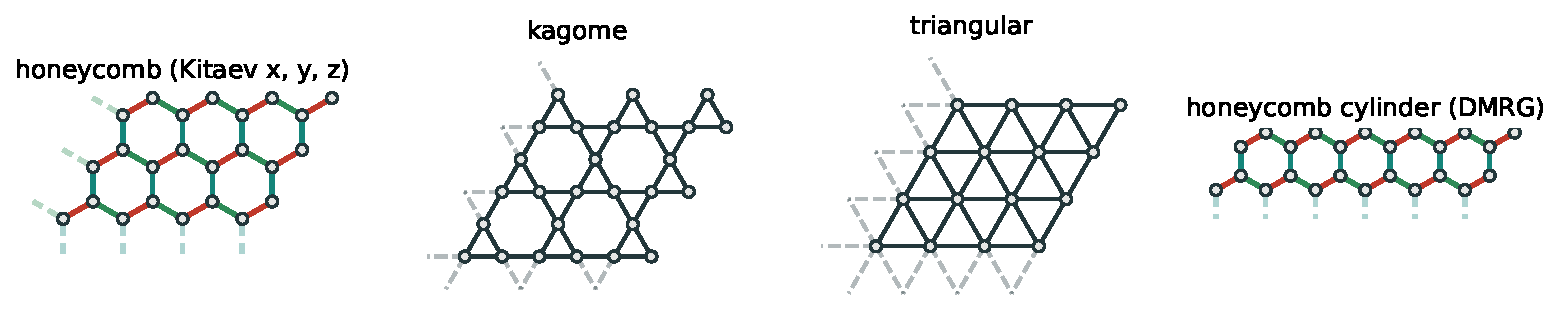
\includegraphics[width=\textwidth]{figs/lattices.pdf}
\vspace{2pt}
\begin{columns}[T]
\column{0.32\textwidth}\small\textbf{Bonds}\\ every infinite-lattice bond mapped once; multi-bonds on small tori; winding numbers for twists and fluxes
\column{0.32\textwidth}\small\textbf{Clusters}\\ $L_1\times L_2$ with periodic or open boundaries, or a supercell matrix $M$ (e.g.\ the $\sqrt{12}\times\sqrt{12}$ cluster that contains both K and M)
\column{0.32\textwidth}\small\textbf{Geometry}\\ plaquettes (hexagons, up/down triangles), translations, allowed $\vk$, high-symmetry paths, Marshall sign
\end{columns}
\end{frame}

% =================================================================== ED
\section{Exact diagonalisation}
\begin{frame}{ED engine}\small
\begin{columns}[T]
\column{0.52\textwidth}
\begin{block}{Hilbert-space engineering}\small
\begin{itemize}
\item $S^z$ sectors selected automatically when $[H,S^z_{\rm tot}]=0$
\item \textbf{Lin two-table hash}: $O(1)$ index of fixed-popcount states,
$\;\mathrm{idx}(s)=\text{off}[s_{\rm hi}]+\text{rank}[s_{\rm lo}]$
\item three back ends: multithreaded CSR, matrix-free Numba ``pull'' kernel ($H$ never stored), cuSPARSE on a GPU; large Krylov spaces resolve topological degeneracies
\end{itemize}
\end{block}
\column{0.45\textwidth}
\begin{block}{Observables}\small
\begin{itemize}
\item total spin $S$, momentum $\vk$, any commuting symmetry (e.g.\ $\Fx{W_p}$, Wilson loops) diagonalised inside multiplets
\item $\langle\Sp{\mathbf S_i\cdot\mathbf S_j}\rangle$, $S(\vq)$, dimer and chirality correlations
\item $\rho_A$, entanglement spectrum, von Neumann and Rényi entropies
\item FTLM: $\En{E}(T), C, S, \chi$; continued fraction $S(\vq,\En\omega)$; real-time evolution
\end{itemize}
\end{block}
\end{columns}
\vspace{1pt}
\begin{exampleblock}{Benchmark}\footnotesize
$4\times4$ square Heisenberg: $\En{E_0}=-11.228\,483\,208$ (exact reference), $\vk=(0,0)$, $S=0$; first excitation at $\vk=(\pi,\pi)$, the Anderson tower of states.
\end{exampleblock}
\end{frame}

% =================================================================== Kitaev
\section{Kitaev honeycomb model}
\begin{frame}{Kitaev model: Majorana fermions in a static $\mathbb Z_2$ gauge field}
\begin{columns}[T]
\column{0.56\textwidth}
\footnotesize
\[
H=-\sum_{\langle jk\rangle_\alpha}\Cp{K_\alpha}\,\Sp{\sigma^\alpha_j\sigma^\alpha_k}
\;-\;\Cp{\kappa}\!\!\sum_{\langle jkl\rangle}\Sp{\sigma^x_j\sigma^y_k\sigma^z_l}
\]
Kitaev's representation: $\Sp{\sigma^\alpha_j}=i\,\Ga{b^\alpha_j}\Mj{c_j}$, $\;\Ga{u_{jk}}=i\Ga{b^\alpha_j b^\alpha_k}=\pm1$ conserved:
\[
H_{\Ga u}=\frac{i}{4}\sum_{jk}A_{jk}\,\Mj{c_jc_k},\qquad
\begin{aligned}A_{jk}&=2\Cp{K_\alpha}\Ga{u_{jk}}\\[-2pt]A_{jl}&=-2\Cp{\kappa}\,\epsilon_{\alpha\beta\gamma}\Ga{u_{jk}u_{kl}}\end{aligned}
\]
\[
\En{E_0}(\Ga u)=-\tfrac12\sum_m\En{\varepsilon_m},\qquad \pm\En{\varepsilon_m}=\mathrm{eig}(iA)
\]
Fluxes $\Fx{W_p}=\prod_{\langle jk\rangle\in p}\Ga{u_{jk}}$: the ground state is flux-free (Lieb).
\column{0.42\textwidth}
\begin{alertblock}{The hard part: physical states}\footnotesize
The Majorana space is $4^N$; physical states satisfy $D_j=\Ga{b^x_jb^y_jb^z_j}\Mj{c_j}=1$.
qslab evaluates $\prod_j D_j$ \textbf{numerically}:
\[
\prod_j D_j = s_{\rm perm}\,(-1)^{N/2}\prod_{\langle jk\rangle}\Ga{u_{jk}}\;\mathrm{sgn\,Pf}(A_{\Ga u})
\]
$s_{\rm perm}$ is the sign of reordering all $4N$ Majoranas, and the Pfaffian gives the matter-vacuum parity.
No lattice-specific formula is needed, so it works on any torus or tilted cluster.
\end{alertblock}
\end{columns}
\end{frame}

\begin{frame}{Exact projection reproduces the full ED spectrum, level by level}
\begin{columns}[c]
\column{0.5\textwidth}
\centering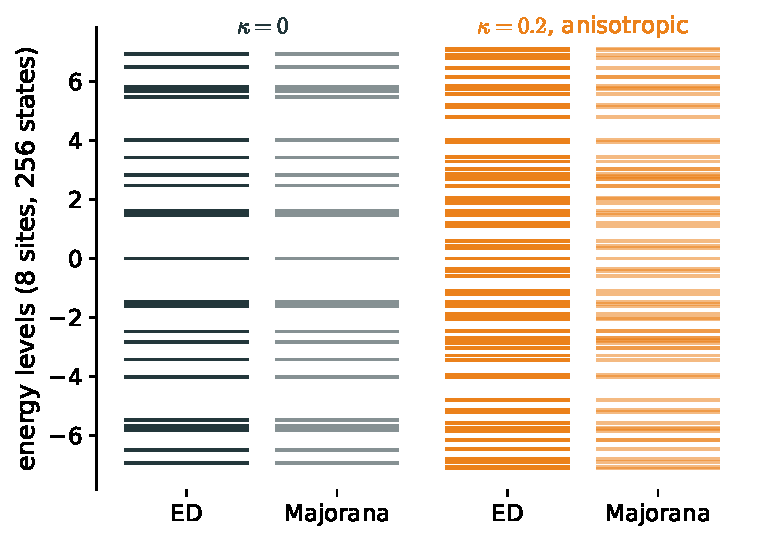
\includegraphics[width=\textwidth]{figs/kitaev_validation.pdf}
\column{0.47\textwidth}
\small
\begin{itemize}
\item 8 sites: every one of the 256 eigenvalues is recovered, for all $2^{12}$ gauge configurations $\times$ occupations of the right parity
\item uniform gauge multiplicity $2^{N-1}=128$, including the $\Cp\kappa$ term and anisotropic $\Cp{K_\alpha}$
\item 18 sites: $\En{E_0}^{\rm Maj}=-14.291\,502\,62$ against $\En{E_0}^{\rm ED}=-14.291\,502\,62$
\end{itemize}
\begin{exampleblock}{Thermodynamic limit}\small
$\En{E_0}/N=-0.787\,30\,\Cp K$ (Pauli units) $=-0.196\,82\,|\Cp K|$ (spin units)\\
NN correlation $\langle\Sp{\sigma\sigma}\rangle=0.5249$; all longer-range spin correlations vanish exactly\\
vison pair $\Delta_v=0.265\,\Cp K$
\end{exampleblock}
\end{columns}
\end{frame}

\begin{frame}{Majorana bands, phase diagram and the chiral phase}
\centering
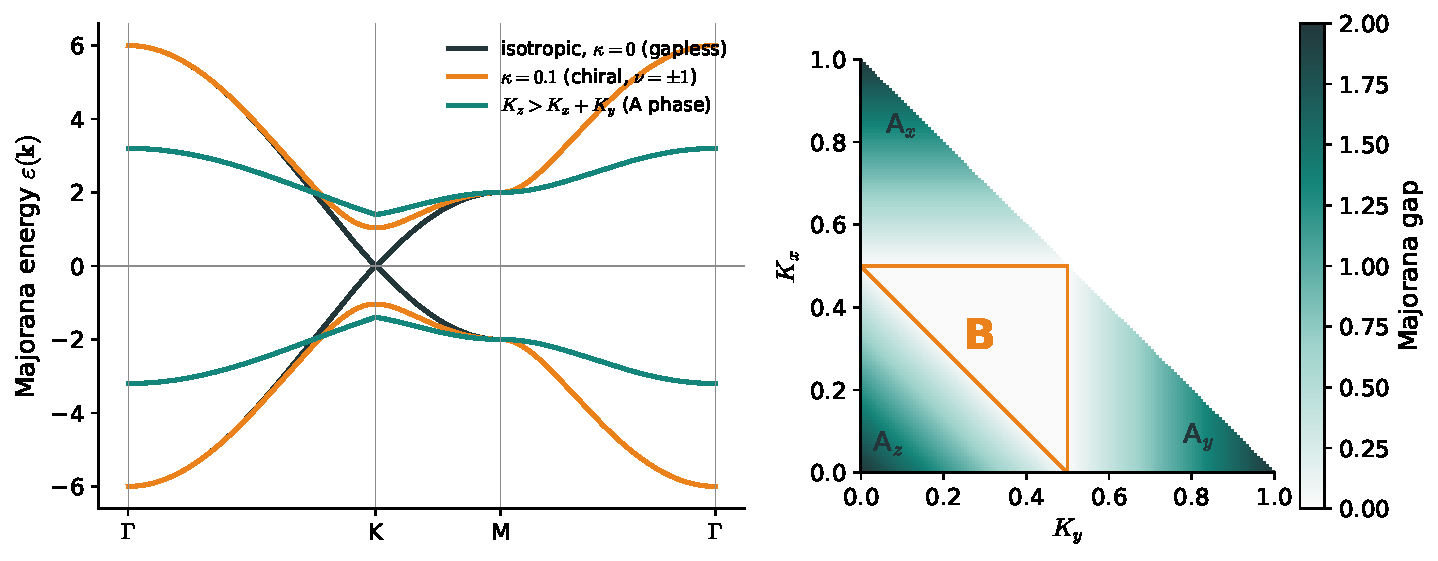
\includegraphics[width=0.8\textwidth]{figs/kitaev_bands_phase.pdf}
\footnotesize
\[
\En{\varepsilon}(\vk)=\sqrt{|f(\vk)|^2+\Delta(\vk)^2},\quad f=2\sum_\alpha \Cp{K_\alpha}e^{i\vk\cdot\mathbf d_\alpha},\quad
\Delta=4\Cp\kappa\left[\sin\vk\!\cdot\!\mathbf a_1-\sin\vk\!\cdot\!\mathbf a_2+\sin\vk\!\cdot\!(\mathbf a_2-\mathbf a_1)\right]
\]
Fukui--Hatsugai--Suzuki Chern number $\nu=\mp1$ for $\Cp\kappa\gtrless0$: non-Abelian Ising anyons and half-quantised $\kappa_{xy}/T$.
\end{frame}

\begin{frame}{Finite temperature: sign-free Majorana Monte Carlo}
\centering
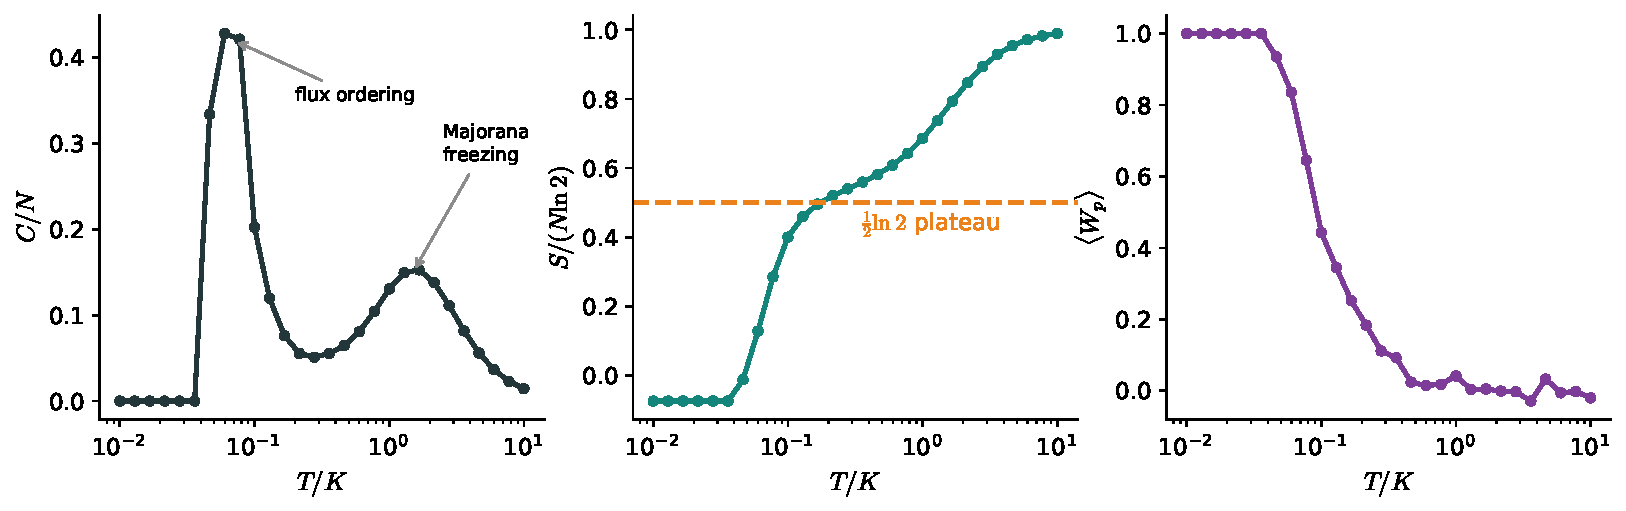
\includegraphics[width=0.93\textwidth]{figs/kitaev_thermo.pdf}
\begin{columns}[T]
\column{0.55\textwidth}\footnotesize
Metropolis over $\Ga{u_{jk}}$ with the exact free-fermion weight
$F_{\Ga u}=-T\sum_m\ln\!\left[2\cosh(\En{\varepsilon_m}/2T)\right]$ (Nasu, Udagawa, Motome 2014).
Each temperature is an independent chain, run in parallel with \texttt{pmap} on processes or MPI ranks.
\column{0.42\textwidth}\footnotesize
Two energy scales: itinerant Majoranas freeze at $T_H\approx1.5\Cp K$, fluxes order at $T_L\ll T_H$.
In between the entropy sits on the $\tfrac12\ln2$ plateau.
\end{columns}
\end{frame}

% =================================================================== materials
\section{Kitaev materials}
\begin{frame}[fragile]{J--K--$\Gamma$--$\Gamma'$--J$_3$: from $\alpha$-RuCl$_3$ to model to numbers}
\begin{columns}[T]
\column{0.55\textwidth}\small
On a $\gamma$-bond ($\alpha,\beta$ the other two labels):
\[
\begin{aligned}
H_{ij}=\;&\Cp J\,\Sp{\mathbf S_i\!\cdot\!\mathbf S_j}+\Cp K\,\Sp{S^\gamma_iS^\gamma_j}
+\Cp\Gamma\,(\Sp{S^\alpha_iS^\beta_j+S^\beta_iS^\alpha_j})\\
&+\Cp{\Gamma'}(\Sp{S^\gamma_iS^\alpha_j+S^\alpha_iS^\gamma_j+S^\gamma_iS^\beta_j+S^\beta_iS^\gamma_j})
\end{aligned}
\]
plus $\Cp{J_3}$ and $-g\,\Cp{\mathbf h}\cdot\sum\Sp{\mathbf S_i}$.

\vspace{3pt}
\begin{tabular}{@{}lccc@{}}\toprule
12 sites & $\En{E}/N$ & gap & $\langle\Fx{W_p}\rangle$\\\midrule
FM Kitaev & $-0.2042$ & -- & conserved\\
$K+\Gamma$ & $-0.3417$ & 0.139 & $-0.21$\\
RuCl$_3$-like & $-0.3809$ & 0.094 & $-0.22$\\\bottomrule
\end{tabular}

\vspace{3pt}
At the RuCl$_3$-like point $S(\vq)$ peaks at \textbf{M}: zigzag correlations.
\column{0.42\textwidth}
\begin{block}{From DFT to model}\small
DFT+SOC $\to$ Wannier90 ($t_{2g}$/$j_{\rm eff}$) $\to$ $3\times3$ exchange tensors $\to$ \texttt{qslab.exchange(i, j, J)}
\end{block}
\begin{lstlisting}
pars = dict(J=-0.1, K=-1, Gamma=0.5,
            Gamma_p=-0.025, J3=0.1)
H = models.kitaev_heisenberg_gamma(
        lat, **pars, h=h*n111)
d = DMRG(H, lat.N, chi_max=400)  # complex MPO
\end{lstlisting}
\small $\Cp\Gamma$ terms make the MPO complex; qslab writes $\Sp{\sigma^y}=-i\,Y_r$ with real $Y_r$, so the MPO stays real whenever it can.
\end{columns}
\end{frame}

% =================================================================== toric
\section{Toric code and topological entanglement}
\begin{frame}{Toric code: degeneracy, anyons, and $\gamma=\ln 2$ on thousands of qubits}
\begin{columns}[T]
\column{0.38\textwidth}\footnotesize
\[
H=-\Cp{J_e}\sum_s\prod_{e\in s}\Sp{\sigma^x_e}-\Cp{J_m}\sum_p\prod_{e\in p}\Sp{\sigma^z_e}
\]
\begin{itemize}
\item ED ($L=3$): $\En{E_0}=-18$, 4-fold degenerate; Wilson loops $(\Fx{Z_1},\Fx{Z_2})=(\pm1,\pm1)$
\item $e$ and $m$ pairs cost $4\Cp J$; string length is free (deconfined)
\item stabilizer formalism:\\
$\Et{S_A}/\ln2=\mathrm{rank}_{\rm GF(2)}(G|_A)-|A|$
\end{itemize}
\[
\begin{aligned}-\Et\gamma=\;&\Et{S_A}+\Et{S_B}+\Et{S_C}\\&-\Et{S_{AB}}-\Et{S_{BC}}-\Et{S_{CA}}+\Et{S_{ABC}}\end{aligned}
\]
\column{0.6\textwidth}
\centering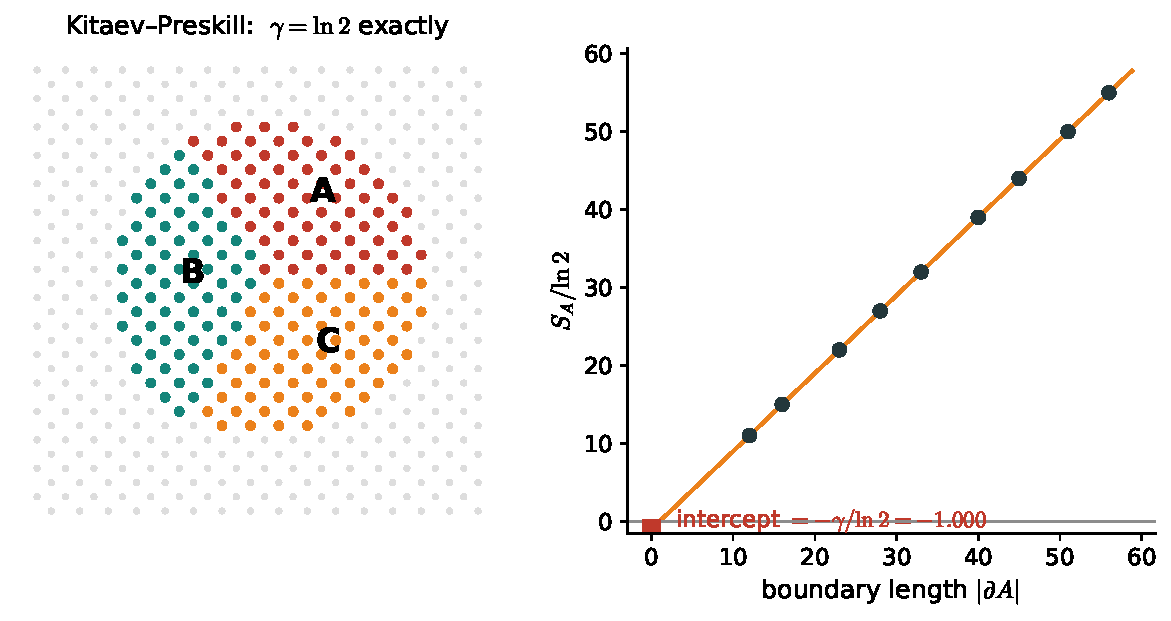
\includegraphics[width=\textwidth]{figs/toric_tee.pdf}\\
\small Kitaev--Preskill and Levin--Wen both give $\Et\gamma=\ln2$ to machine precision for $L=8$--$28$.
\end{columns}
\end{frame}

% =================================================================== kagome
\section{Frustrated Heisenberg magnets}
\begin{frame}{Kagome antiferromagnet: no order, many singlets, Dirac spinons}
\centering
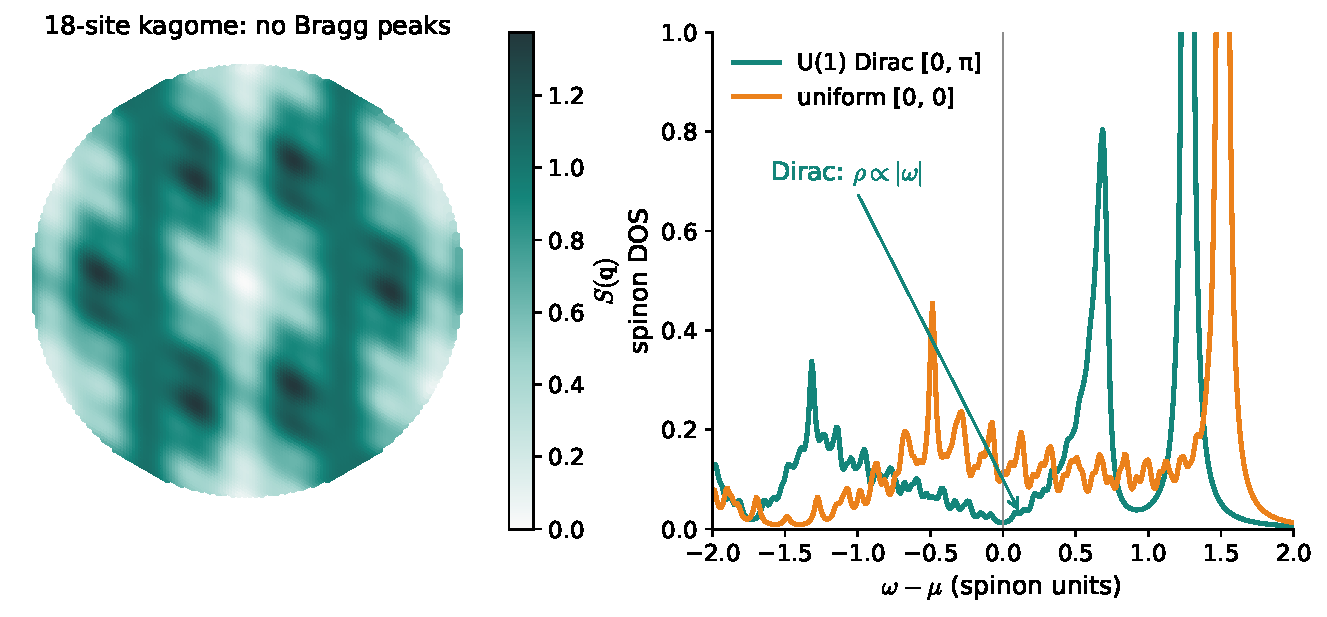
\includegraphics[width=0.76\textwidth]{figs/kagome_sq_dos.pdf}\\\footnotesize
\begin{columns}[T]
\column{0.5\textwidth}
ED: $N=12$, $\En{E_0}/N=-0.4537$, $\Delta_T=0.383$; $N=18$, $-0.4471$, $\Delta_T=0.285$, with 7 singlets below the first triplet.
\column{0.47\textwidth}
U(1) Dirac spin liquid: flux $0$ through triangles and $\pi$ through hexagons, so $\rho(\En\omega)\propto|\En\omega|$.
\end{columns}
\end{frame}

\begin{frame}{Triangular J$_1$--J$_2$: from 120\textdegree{} order to a spin liquid}
\centering
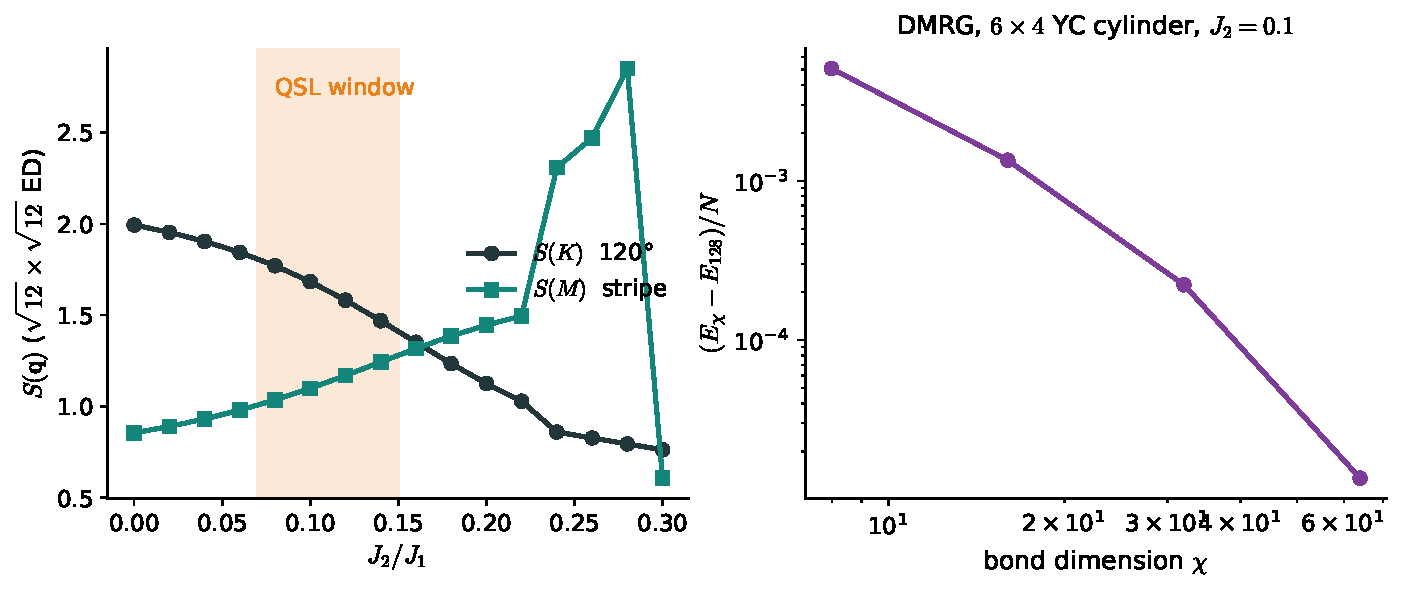
\includegraphics[width=0.78\textwidth]{figs/triangular.pdf}
\footnotesize
\begin{columns}[T]
\column{0.5\textwidth}
ED on the tilted $\sqrt{12}\times\sqrt{12}$ cluster, which contains both K and M. $S(\mathrm K)$ collapses entering the spin-liquid window $0.07\lesssim \Cp{J_2}/\Cp{J_1}\lesssim0.15$, and $S(\mathrm M)$ grows beyond it.
\column{0.47\textwidth}
DMRG on YC cylinders with automatic MPOs: energy converges exponentially in $\chi$. The scan runs in parallel with \texttt{qslab.pmap}.
\end{columns}
\end{frame}

% =================================================================== partons
\section{Partons, Gutzwiller projection, VMC}
\begin{frame}{Partons: any flux pattern on any cluster}
\begin{columns}[T]
\column{0.53\textwidth}\footnotesize
\[
\Sp{\mathbf S_i}=\tfrac12 f^\dagger_i\Sp{\bm\sigma}f_i,\qquad
H_{\rm MF}=-\sum_{\langle ij\rangle}\left(\chi_{ij}f^\dagger_{i}f_{j}+\text{h.c.}\right)
\]
\textbf{Flux solver.} With $D$ the oriented plaquette--bond incidence matrix,
\[
D\,\theta=\Fx{\Phi}\pmod{2\pi}
\]
is solved by GF(2) elimination (real $0/\pi$ ansätze) or least squares (chiral ansätze). Twisted boundaries close the Fermi shell.

\vspace{3pt}
\textbf{Projection.} $|\Wf\psi\rangle=P_G|\mathrm{FS}\rangle$,
\[
\Wf\psi(\Sp\sigma)=\mathrm{sgn}(\Sp\sigma)\,\det\Phi_{\uparrow}\,\det\Phi_{\downarrow}
\]
evaluated exactly ($N\lesssim24$) or by VMC with $O(1)$ ratios $G=\Phi M^{-1}$ and Sherman--Morrison updates.
\column{0.44\textwidth}
\centering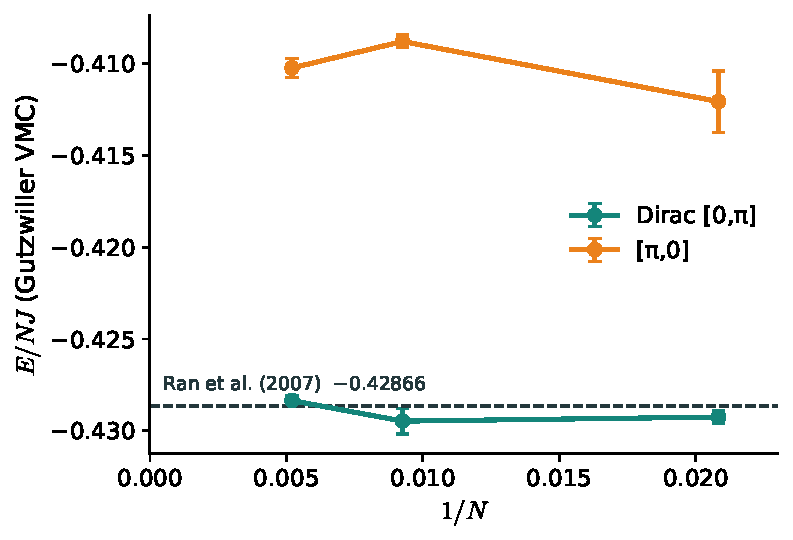
\includegraphics[width=0.9\textwidth]{figs/kagome_vmc.pdf}
\begin{exampleblock}{Cross-checks}\scriptsize
$\pi$-flux $4\times4$: VMC $-0.63769(35)$ against exact projection $-0.637730$\\
Kagome DSL, 108 sites: $-0.4291(9)$, literature $-0.42866$
\end{exampleblock}
\end{columns}
\end{frame}

% =================================================================== DMRG + NQS
\section{DMRG and neural quantum states}
\begin{frame}{DMRG with automatic MPOs \;$\cdot$\; RBM neural quantum states}
\begin{columns}[T]
\column{0.48\textwidth}
\begin{block}{Two-site DMRG}\footnotesize
\begin{itemize}
\item MPO built from \emph{any} 1- and 2-site \texttt{Operator}, with channels shared per (start site, operator); bond dimension $2+n_{\rm open}$, long-range cylinder bonds handled
\item restarted Lanczos with full reorthogonalisation; SVD truncation with $\chi$ schedules
\item $\Et{S}$ on every bond, entanglement spectrum, correlation matrices in $O(N^2\chi^3)$, energy variance
\item NumPy/BLAS on all cores, or CuPy on a GPU
\end{itemize}
\end{block}
\footnotesize DMRG = ED to $10^{-8}$ on triangular, honeycomb $\Gamma$ and $4\times4$ torus tests.
\column{0.5\textwidth}
\footnotesize
\[
\Wf\psi(\Sp{s})=e^{\sum_i a_i\Sp{s_i}}\prod_j 2\cosh\!\Big(b_j+\sum_iW_{ji}\Sp{s_i}\Big)
\]
Stochastic reconfiguration: $\delta p=-\eta\,(S+\epsilon)^{-1}F$, exact sums or Metropolis; under MPI, gradients are averaged with \texttt{allreduce}.\par\vspace{2pt}
\centering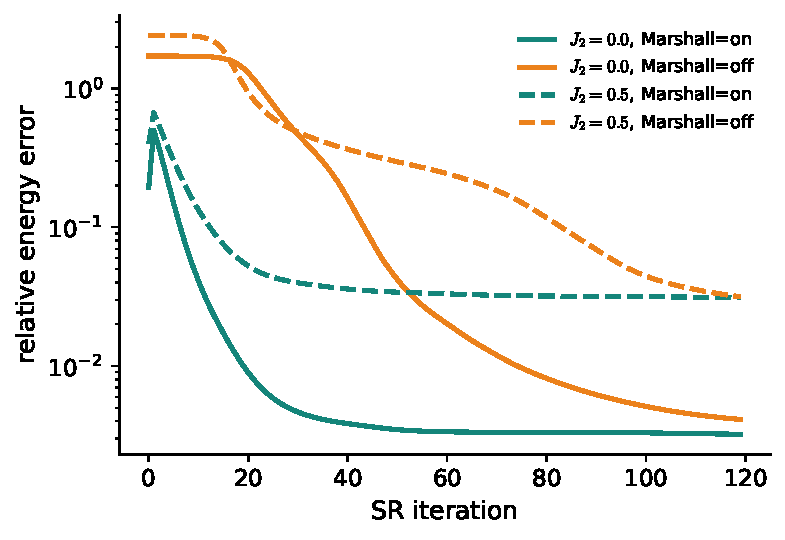
\includegraphics[width=0.64\textwidth]{figs/nqs.pdf}\\
\scriptsize The Marshall sign speeds convergence by about $3\times$. At $\Cp{J_2}=0.5$ both runs stall near $3\%$: frustration removes the sign rule.
\end{columns}
\end{frame}

% =================================================================== dynamics
\section{Dynamics and thermodynamics}
\begin{frame}{Fingerprints of fractionalisation}
\centering
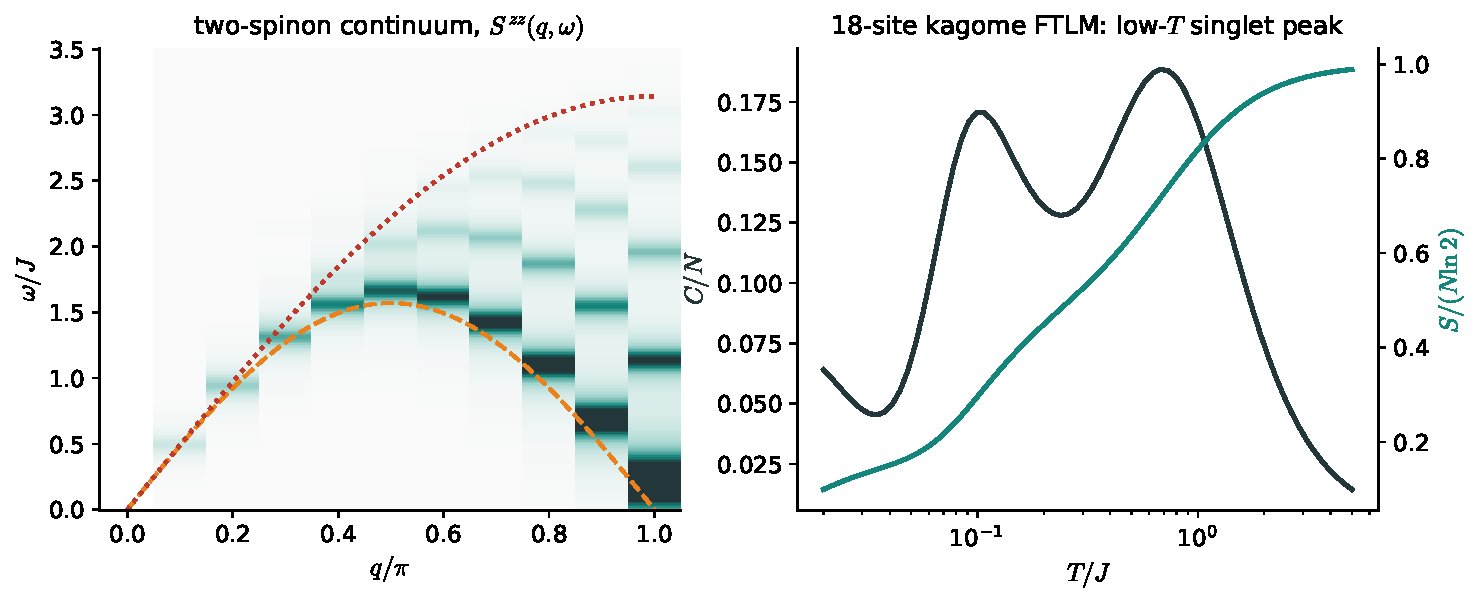
\includegraphics[width=0.8\textwidth]{figs/dynamics_thermo.pdf}
\footnotesize
\begin{columns}[T]
\column{0.5\textwidth}
Continued-fraction Lanczos: $S(\vq,\En\omega)=-\frac1\pi\mathrm{Im}\langle\Wf\psi_0|O^\dagger_{\vq}\frac{1}{\En\omega+\En{E_0}+i\eta-H}O_{\vq}|\Wf\psi_0\rangle$.
The 20-site chain fills the two-spinon continuum between $\frac\pi2|\sin q|$ and $\pi|\sin\frac q2|$.
\column{0.47\textwidth}
FTLM (Jaklič--Prelovšek), parallel over random vectors and $S^z$ sectors, using spin-flip symmetry.
The 18-site kagome cluster shows a low-$T$ singlet peak below the main peak.
\end{columns}
\end{frame}

% =================================================================== parallel
\section{Parallel computing}
\begin{frame}[fragile]{From a laptop to a node, many nodes, or a GPU, with one code}
\begin{columns}[T]
\column{0.56\textwidth}
\footnotesize
\begin{tabularx}{\linewidth}{@{}>{\bfseries}l>{\raggedright\arraybackslash}p{2.0cm}>{\raggedright\arraybackslash}X@{}}\toprule
level & enabled by & what runs in parallel\\\midrule
\rowcolor{tealx!8}threads & Numba, BLAS (default) & ED mat-vec (CSR or matrix-free), DMRG, VMC algebra\\
processes & \texttt{pmap} (default) & sectors, FTLM vectors, scans, MC temperatures\\
\rowcolor{orangex!8}MPI & \texttt{mpi4py} (optional) & tasks across nodes; VMC/NQS/MC chains with \texttt{allreduce}\\
GPU & CuPy (optional) & ED, Lanczos, DMRG tensors, Majorana diagonalisation\\\bottomrule
\end{tabularx}

\vspace{2pt}
The Numba ``pull'' kernel needs no atomics, because each thread owns its output rows:
\[
(H v)_m=\sum_{\text{fmask}}\;\mathrm{amp}(m\oplus\text{fmask})\;v_{\mathrm{idx}(m\oplus\text{fmask})}
\]
\column{0.41\textwidth}
\begin{lstlisting}
# same script everywhere
res = qslab.pmap(point, J2_grid)

# one node
QSLAB_NUM_THREADS=128 python run.py
# many nodes
srun -N 8 --ntasks-per-node=8 \
  python run.py
# GPU
QSLAB_BACKEND=gpu python run.py
\end{lstlisting}
\small SLURM scripts for Ibex and Shaheen are in \texttt{examples/}.
\texttt{qslab-info} prints the detected threads, MPI ranks and GPU.
\end{columns}
\end{frame}

% =================================================================== validation
\section{Validation, tutorials and quizzes}
\begin{frame}{Validation: 21 benchmark tests}
\small
\begin{tabularx}{\textwidth}{@{}lXr@{}}\toprule
check & reference & qslab\\\midrule
$4\times4$ Heisenberg & $-11.228\,483\,208$ & \ok\ exact\\
Kitaev, 8 sites, full spectrum ($\Cp\kappa=0, 0.2$) & ED & \ok\ all levels\\
Kitaev, 18 sites & ED $-14.291\,502\,6$ & \ok\ $10^{-8}$\\
Kitaev TL, vison pair, Chern & $-0.7873$, $\approx0.26$, $\pm1$ & \ok\\
Toric code ED $L=3$ & $4\times(-18)$, gap 4 & \ok\\
Topological EE (KP, LW) & $\ln2$ & \ok\ exact\\
$\pi$-flux VMC $4\times4$ & exact projection $-0.637\,730$ & $-0.63769(35)$\\
Kagome Dirac SL & $-0.428\,66$ (Ran et al.) & $-0.4291(9)$\\
DMRG (triangular, complex $\Gamma$ cylinder) & ED & \ok\ $10^{-8}$\\
NQS chain $L=8$ & ED & $<1\%$\\
FTLM $C(T)$, $\En E(T)$ & full diagonalisation & \ok\\
pmap: serial, thread, process, MPI (2 ranks) & identical results & \ok\\\bottomrule
\end{tabularx}
\end{frame}

\begin{frame}[fragile]{Eight executed tutorials and seven quizzes}
\begin{columns}[T]
\column{0.5\textwidth}\small
\begin{enumerate}
\item getting started and parallel computing
\item Kitaev honeycomb: ED $\to$ Majorana $\to$ MC
\item toric code: anyons and $\Et\gamma=\ln 2$
\item kagome: ED, partons, chiral SL, DMRG
\item triangular J$_1$--J$_2$: $\sqrt{12}$ scan and cylinders
\item square J$_1$--J$_2$: benchmarks, $\pi$ flux, NQS
\item Kitaev materials: RuCl$_3$, fields, DFT link
\item dynamics and thermodynamics
\end{enumerate}
\column{0.47\textwidth}
\begin{lstlisting}
from qslab import quiz
quiz.topics()
# kitaev, toric_code, kagome, triangular,
# square_j1j2, kitaev_heisenberg_gamma,
# methods
quiz.run("kitaev")          # interactive
quiz.check("kitaev", 4, -0.7873)
\end{lstlisting}
\small
Conceptual multiple-choice questions plus \textbf{computational} questions answered by running qslab; every reference number was produced by the benchmarked solvers.
\vspace{4pt}\colorbox{softbg}{\scriptsize\texttt{\$ qslab-quiz kagome}}
\end{columns}
\end{frame}

\begin{frame}[fragile]{Get started}
\begin{columns}[T]
\column{0.5\textwidth}
\begin{lstlisting}[language=bash]
git clone https://github.com/Gokaran-Shukla/qslab
cd qslab
pip install -e ".[fast,mpi]"   # numba + mpi4py
pip install cupy-cuda12x        # optional GPU
pytest                          # 21 tests
jupyter lab tutorials/
\end{lstlisting}
\vspace{4pt}
\small\textbf{Scope.} ED to about 30 spins on a large node (shared memory). The DMRG is a reference implementation without U(1)/SU(2) blocks; for production cylinders of width $\ge8$, cross-check with TeNPy, ITensor or block2. VMC covers U(1) parton ansätze.
\column{0.47\textwidth}
\begin{block}{Take-home}\small
\begin{itemize}
\item one Pauli-string \texttt{Operator}, six solvers, consistent conventions
\item Kitaev physics solved \emph{exactly}, with exact projection, and checked against ED
\item topology ($\Et\gamma$), fractionalisation ($S(\vq,\En\omega)$, $C(T)$) and ansätze (VMC) in one place
\item scales from a laptop to multi-node and GPU runs, with the same script
\end{itemize}
\end{block}
\centering\small
\href{https://github.com/Gokaran-Shukla/qslab}{\texttt{github.com/Gokaran-Shukla/qslab}}\quad$\cdot$\quad MIT licence
\end{columns}
\end{frame}

\appendix
\begin{frame}[standout]
Thank you\\[6pt]
\normalsize\texttt{pip install -e ".[fast,mpi]"}\quad$\cdot$\quad\texttt{qslab.quiz.run("kitaev")}
\end{frame}

\end{document}
